Whenever tasks become more extensive and complex, systems react with division of work and specialization. By subdividing into smaller, less complex tasks, large processes can be distributed and processed in parallel, and at the same time the executing components are more efficient because they have to cover less noise, peripheral cases and side aspects. We can observe this development on different scales in computer science. At the hardware level, computations are distributed from general-purpose CPUs to GPUs, digital signal processors (DSPs) or other adapted hardware, and the concrete hardware logic is abstracted from the program logic to be executed. At the software level, components are separated both vertically, i.e. between business logic, language runtime environment and operating system services, and horizontally, i.e. between components of the different levels of independence. \\

Besides improved efficiency and scalability, compartmentalization has also a major advantage when it comes to security. Separation of concerns and minimization of trust assumptions are core concepts in defense in depth for cloud deployments. \seflue{"core concepts in defense in depth for cloud deployments" ... K\"ommer das nochmal umschreiben, ich raffs nicht.} But again they are likewise seen on the scale of single machines. A cloud deployment consisting of one big trust zone protected by a perimeter is the large scale equivalent of a monolithic kernel, with unrestricted memory access among all kernel space processes. The problem with this is clearly evident in monolithic Unix kernels. Despite various measures to prevent unauthorized memory access (e.g. control flow integrity and data execution prevention) or to make it more difficult to exploit security vulnerabilities (e.g. address space layout randomization and stack canaries), according to statistics of the NIST\cite{nvd} the number of vulnerabilities in the kernel ecosystem is still increasing. An analysis of the NIST National Vulnerability Database in \cite{mckee2022novel} looked at the reasons for critical vulnerabilities over the last 5 years and concluded that 34\% of them were due to lack of storage security, and another 43\% were due to lack of compartimentalization. The authors also pointed out that these vulnerabilities could have been prevented if essentially independent processes could not access shared memory, but that however the so-called least-privilege policy is not enforced by the Linux kernel or other big open source projects as OpenSSL or the Apache Server. 
Similarly, as the authors report in \cite{kirth2022pkru}, the majority of known vulnerabilities in Windows, Chrome and the Android Open Source Project (AOSP) can also be traced back to insecure memory access. \\

So obviously it is desirable to have compartmentalization and data locality enforcement not only in cloud setting but also in the kernel itself. Existing solutions for memory protection are tied to specific hardware requirements as Memory Protection Keys, Trusted Execution Environments like ARMs Trust Zone\cite{pinto2019demystifying} or Intels SGX \cite{costan2016intel} or specific virtualization layers (\cite{tan2007ikernel}, \cite{nikolaev2013virtuos}) and in general require manual code adaptations. The costs of adapting tends to make migration between architectures and to newer solutions more difficult and leads to components being subdivided more coarsely than would make sense in order to save effort and runtime costs. Also in terms of security, compartmentalization and in particular concurrency comes at a cost. Recent trends in secure computing are strongly moving away from simple testing towards verification and proving. This applies to the proof of certain properties of user programs as well as to the verification of compilers, kernels ,or operating systems (e.g. CompCert\cite{leroy2009formal},\cite{sL4Verf}, \cite{gu2016certikos}). Distributed, concurrent programs, however, are much more difficult to verify. \\

While certain costs are unavoidable when program parts are isolated, the costs of manually adapting to different isolation mechanisms are not among them. The classic approach to separating concrete run-time implementations from program logic is compilers. They allow the programmer to define and test the logic within specific programming models and automatically translate and add to them to fit the chosen runtime environment and architecture. 

This work will therefore also be based on Ohua\cite{ertel2015ohua}, a compiler developed to identify independent processing steps from sequential programs and deploy them to concurrent, potentially isolated nodes of a data flow graph. Ohua works on subsets of high-level languages such as Python or Rust. Instead of machine code, Ohua extracts a dataflow program from the input, introducing two main abstractions, the notion of an independent node and the notion of communication edges, and replaces them with the corresponding implementations for different run times. The idea of this work is to use and extend Ohuas capabilities for program transformation. We want to be able to extract isolated components from a shared memory program suitable for unikernels and automatically derive the code to deploy them in a microkernel setting. Concretely we will use the \md operating system as an example backend to provide process isolation. 

The key question we need to answer is: What transformations are needed to turn a monolithic or unikernel program into one in which isolated states work together in a data flow graph? 

A good example case to approach the answer to this question is are server applications. They are quasi-ubiquitous in distributed applications and consist of various components, in particular the data backend, the TCP/IP-Stack and a network driver that should be isolated from each other for security reasons. To better understand the starting point and requirements of this work, in Chapter~\ref{Chapter:Background} we first consider the function of Ohua and the properties of the target architecture \md. Certain properties of Rust's type system are explained in this chapter, as they form the basis of Rust's storage security and are helpful constraints for meaningful transformations. On this basis, Section~\ref{Chapter:Implementation} first describes the example application. In a rough sketch, we first approach the structural problems and describe schematically how the application should function after the transformations. We then describe how individual aspects of the code must be transformed.
One of the main problems we need to solve is how to achieve state locality. Obviously the components of a 

\begin{itemize}
    \item develop and verify the sequential, local code \means have verified transformations applied \means get a verified distributed program with isolation boundaries inserted automatically
\end{itemize}

Actual Problem description

    \begin{enumerate}
        \item Transformation to message passing: In it's current state, smoltcp actually combines the TCP/IP stack and an interface to the actual physical layer. The according parts of the library are coupled via shared references and invoke each other via normal function calls. This works well in unikernels, as well as in monoliths (implemented in user space vs. kernel space respectively). In a microkernel, we might want to separate this two functionalities to use and scale them independently. This requires components to interact not via function calls and shared references but via IPC. So one aspect of the problem is to investigate which constraints the isolation of components imposes on the code and which transformations achieve a compatible structure. 
        \item Local State: Smoltcp is a good example for an application with interacting states. From a bird's eye view we can basically distinguish three states, the server application holding e.g. requests currently to process, the network stack holding for example socket states and the network interface abstraction
    
        \item the state locality problem a) write the code such that no internal function will try to access another components state outside the 'flow' b) rewrite it such a way that Ohua identifies the components we want
        
        \item Compile from Uni- to Microkernel \question{$M^3$ already is a Microkernel using smoltcp as a userspace service, so how to describe exactly what's the point here?}
    \end{enumerate}

    \begin{figure}[H]
    \centering
    
    \begin{subfigure}[b]{0.6\textwidth}
         \centering
         \begin{minted}{rust}
   fn somefun() -> i32 {
       let mut mStruct = MS::default();
       let i = mStruct.f();
       let j = mStruct.g();
       calculate(i,j)
   }       
            \end{minted}
         \caption{Multiple calls to a struct}
         \label{multCalls}
     \end{subfigure}
     %\hfill
     \par\bigskip
     \begin{subfigure}[b]{0.6\textwidth}
         \centering
         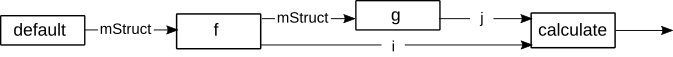
\includegraphics[width=\textwidth]{figures/graph_state_moved.png}
         \caption{Resulting data flow graph}
         \label{DFGStateMoved}
     \end{subfigure}
    \par\bigskip
     \begin{subfigure}[b]{0.6\textwidth}
         \centering
         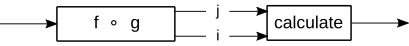
\includegraphics[width=0.6\textwidth]{figures/graph_state_not_moved.png}
         \caption{Target data flow graph}
         \label{DFGStateNotMoved}
     \end{subfigure}
    \caption{}
    \label{fig:SimpleStateUseFigure}
    \end{figure}
    
    \todo[inline]{Explain the contingency from SharedMemory programming model, over M3 to Cloud deployment: maybe Mention in Intro, details in the background}
    Describe essential differences at: 
    \begin{itemize}
        \item Is it one program or do we compile/deploy different programs?  $\rightarrow$ are types known/inferable at compile time/do they have to be? $\rightarrow$ Do we compile for the same OS? \\
         $\Rightarrow$ points above have consequences e.g. 
        \item What are the constraints on types being passed (serializable, are \rust{dyn} allowed, are generics allowed, who takes care of compatibility in case of different OSs)? 
        \item What are other constraints for the programmer (e.g. using system specific interfaces for components) How much packaging does the Compiler have to do (e.g. assorting libraries to components)? 
        \item (How) do we need to handle errors/panics?(in a 'one program' scenario it's one panic to crash them all. How is it in M3? It's even more complex in 'really' distributed scenarios as there are different reasons components might not answer and even if they answer with an error we might have different strategies to handle.)
        \item Do we need to build in a shut down mechanism? 
        \item Can/Should the Compiler be able to detect system interaction and tailor them?        
    \end{itemize}
    
\todo[inline]{Important Point I don't know where to put yet and also needs elaboration:}
\note{The transformation we will extract from the rewriting process are to some degree actually extensions of Ohua programming model. The model currently already enforces 1) variables to be either used as state, or as variable i.e.\means no sending of states and 2) states from outside the loop scope to be only used once inside loop or recursion \means linearity inside loops. What is not enforced currently is that states in general are used only once, i.e. outside loops or when created inside loops states can be used more than once \means so no linearity here.}

    

From the task definition
\begin{itemize}
    \item Implement the cloud-unikernel using SmolTCP, a well-established networking library -> Also schlicht eine Beispielanwendung mit smoltcp, die Anfragen an einen Key-Value-Store handelt. 
    \item Rewrite the unikernel, such that Ohua can compile it Derive and implement transformations to make state usage local to a single program location to provide isolation.
    \item Update existing M3 Backend
    \item Evaluate the approach in the (existing) setup of the YCSB key-value store benchmark along the performance-safety trade-off. 
\end{itemize}

\todo[inline]{Example Rust 4 Unikernel \cite{Rust4Unikernel}}
\todo[inline]{Formal Verification eg for L4 derivatives as motivation \cite{sL4Verf}}

\todo[inline]{Can I get e reference to Compositionality papers .. It would be awesome if we could get the link to \means "we transform a verified object into a verified category, i.e. composable, verified objects"}

\todo[inline]{Certified Concurrent OS in \cite{gu2016certikos} "We have successfully developed a practical concurrent OS kernel and verified its (contextual) functional correctness in Coq. Our certified kernel is written in 6500 lines of C and x86 assembly and runs on stock x86 multicore machines. To our knowledge, this is the first proof of functional correctness of a complete, general-purpose concurrent OS kernel with fine-grained locking."}


